\newpage
\section{PERSONAS}
\subsection{Criação das personas}
As duas personas apresentadas a seguir foram geradas com a ferramenta Claude de IA. Utilizamos a descrição do trabalho e o documento gerado até o sprint 2 para a contextualização no prompt (mostrado adiante), e pedimos a criação de duas personas “aleatórias" para que pudéssemos escrever as suas jornadas. Ainda são protopersonas, pois não foram casos reais, mas foi a opção mais viável para o tempo de entrega do trabalho. Prompt utilizado: "Baseando-se nesta descrição e projeto de software, crie uma persona sênior e uma persona tutor, descreva estas personas para que sejam utilizadas na criação de jornadas de usuário”.

\subsection{Persona Sênior}
\begin{figure}[h]
    \centering
    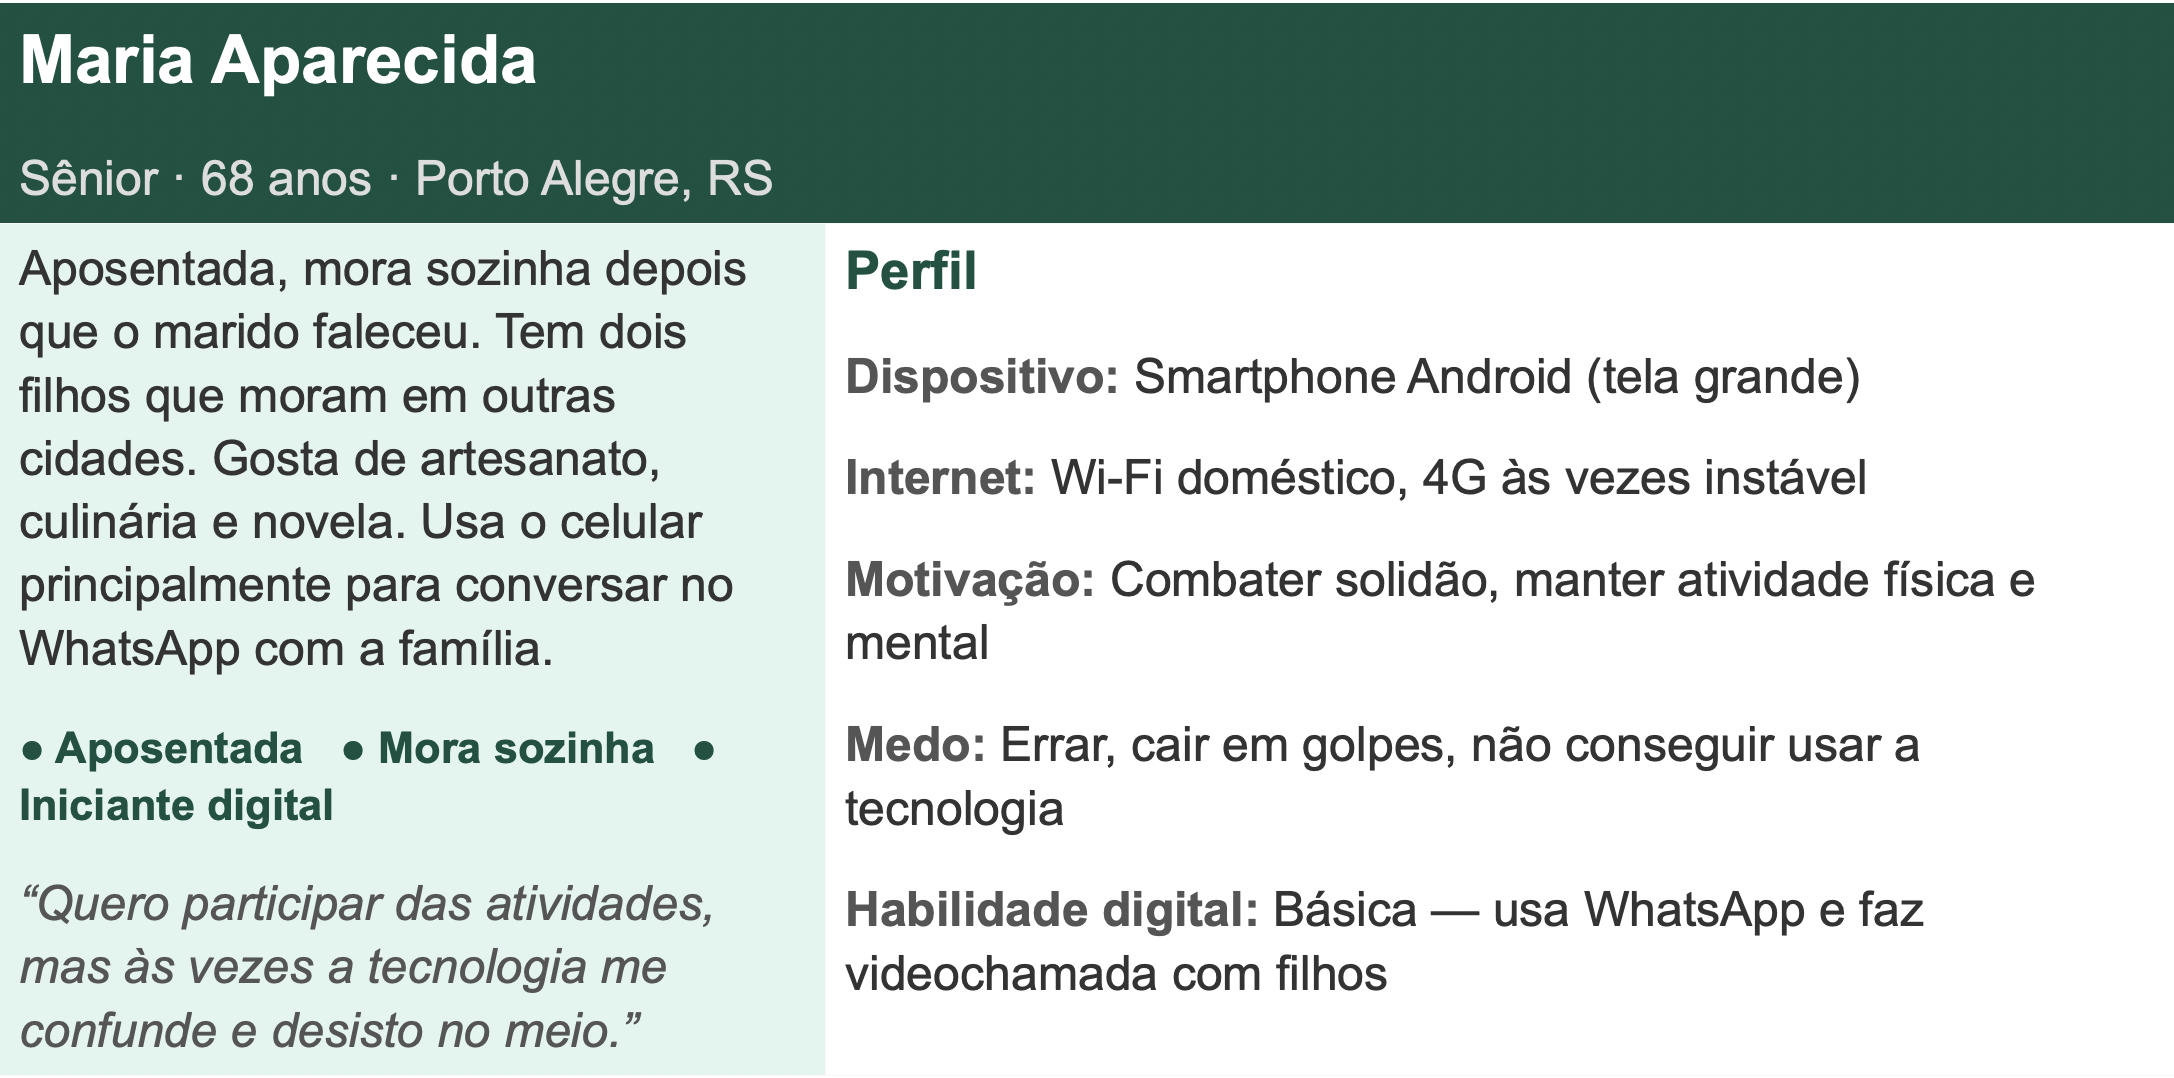
\includegraphics[width=0.75\linewidth]{images/personaSenior.png}
    \label{fig:personaSenior}
\end{figure}

\subsection{Persona Turora}
\begin{figure}[h]
    \centering
    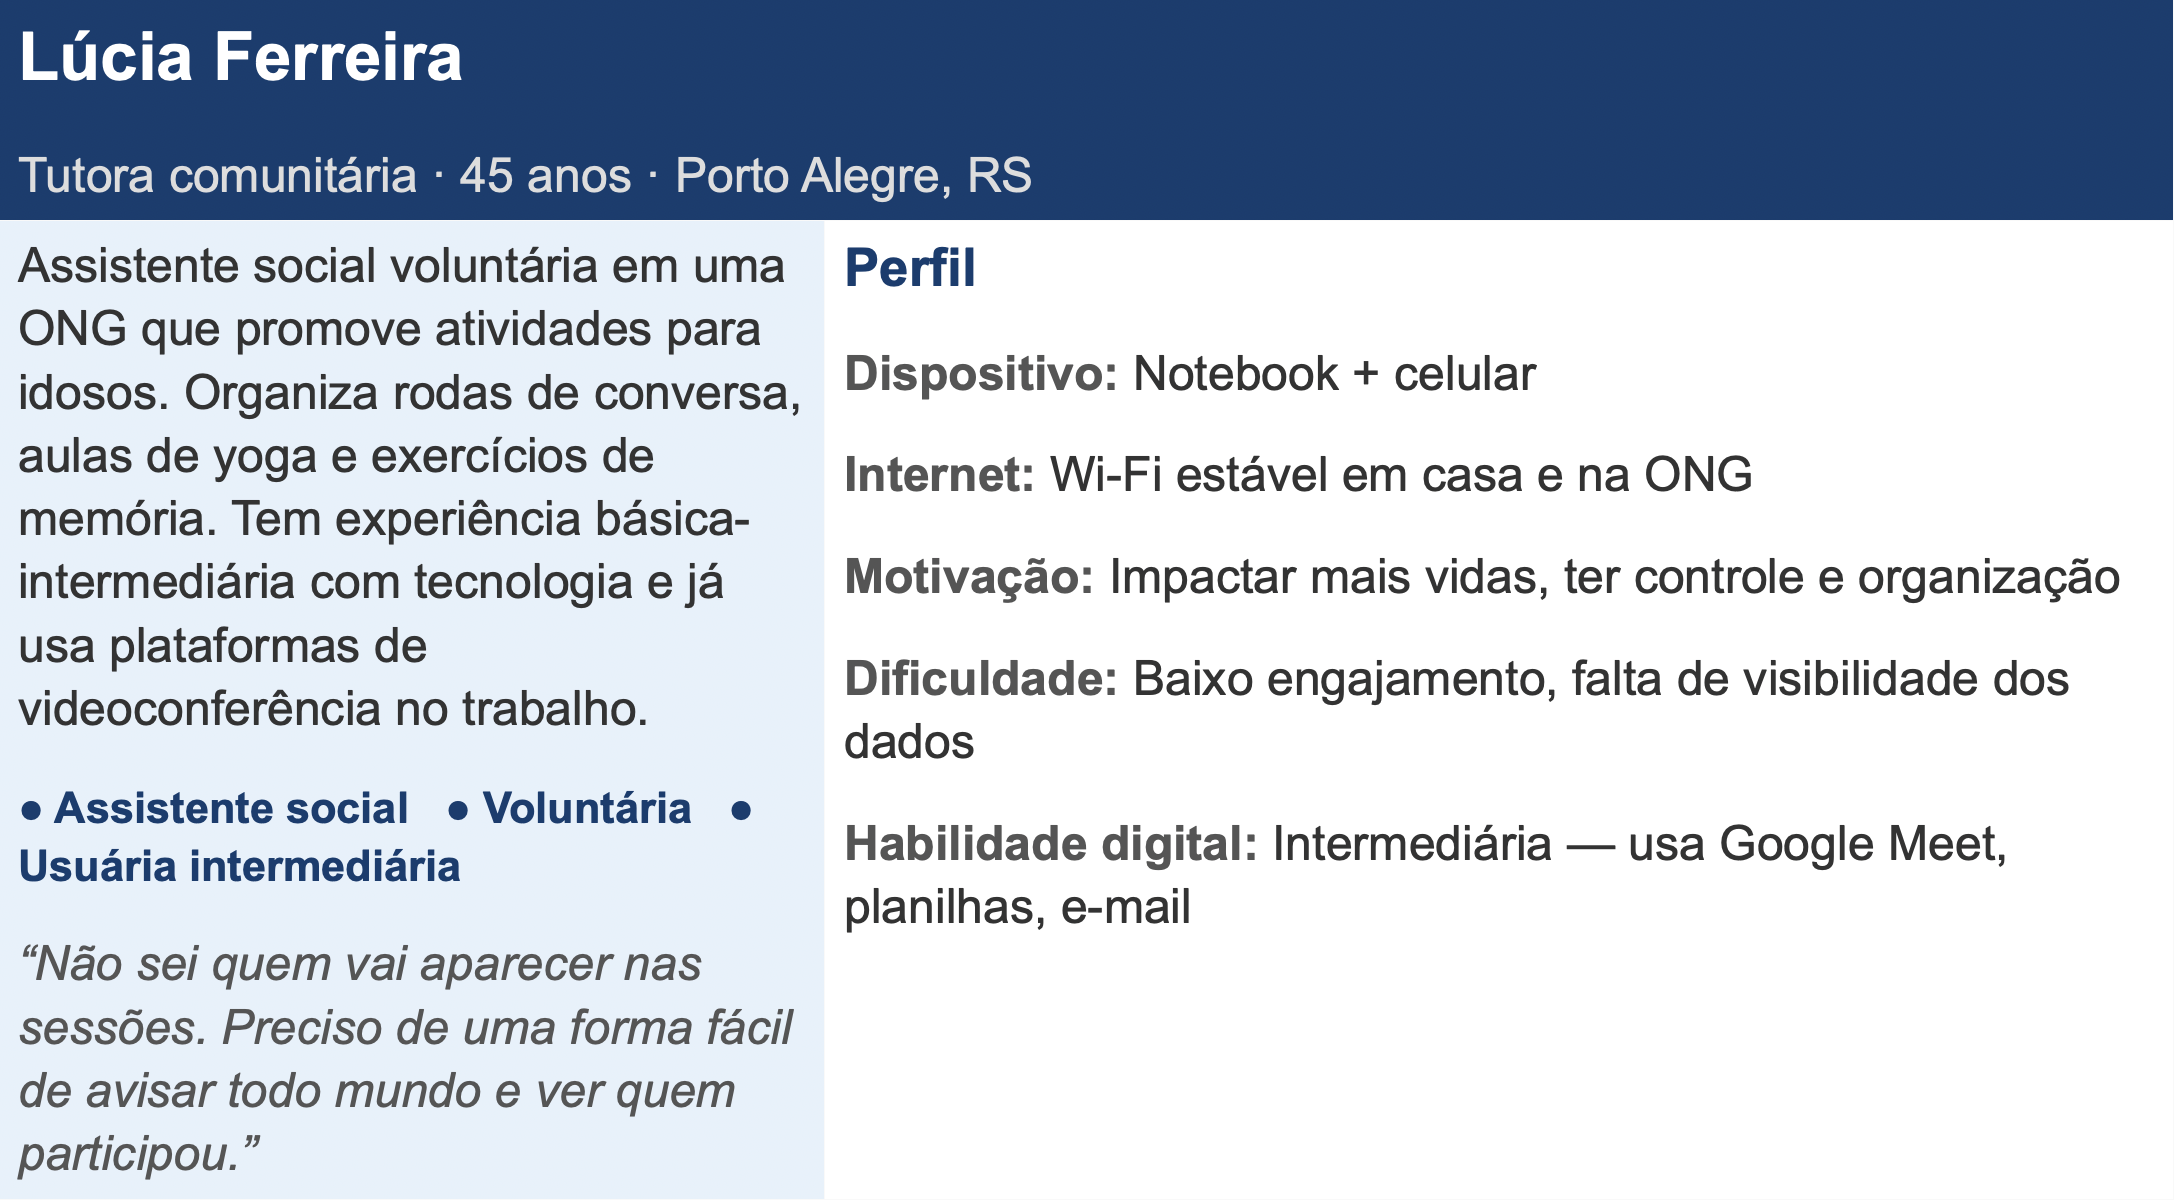
\includegraphics[width=0.75\linewidth]{images/personaTutora.png}
    \label{fig:personaTutora}
\end{figure}
